% TeX file "simulation"

% Master thesis 
% Sven Jacobs
% Winter 2022, M.Sc. Economics, Bonn University
% Supervisor: Prof. Dr. Dominik Liebl


\section{Simulation}

To study the finite-sample performance of the asymptotically valid confidence intervals from Section~\ref{sec:inference},
we conduct a Monte Carlo experiment.
We compare empirical coverage and average interval length for three realistic conditional expectation functions.

\subsection{Setup}

The setup for the simulation study is the same as in \textcite{Calonico_2014},
which itself is based on the data generating process in \textcite{Imbens_2012}.
For each replication the data are generated as $n = 500$ i.i.d.\ draws, $i = 1, \dots, n$, from the model
\begin{align}
	Y_i &= \mu_{j}(X_i) + \varepsilon_i \,, \quad j = 1, 2, 3 \,, \\
	X_i &\sim 2 \Beta(2, 4) -1 \,, \\
	\varepsilon_i &\sim \mathcal{N}(0, 0.1295^2) \,,
\end{align}
where $\Beta(\alpha, \beta)$ denotes the beta distribution with shape parameters $\alpha$ and $\beta$,
and the index $j$ specifies the functional form of the conditional expectation function.
Three models are considered (Figure~\ref{fig:simulation_models}), with the following functional forms:
\begin{align}
	\mu_{1}(x) &=
	\begin{cases}
		0.48 + 1.27x + 7.18x^2 + 20.21x^3 + 21.54x^4 + 7.33x^5 & , x < 0 \\
		0.52 + 0.84x - 3.00x^2 + 7.99x^3 - 9.01x^4 + 3.56x^5   & , x \geq 0
	\end{cases} \,; \\
	\mu_{2}(x) &=
	\begin{cases}
		3.71 + 2.30x + 3.28x^2 + 1.45x^3 + 0.23x^4 + 0.03x^5 	 & , x < 0 \\
		0.26 + 18.49x - 54.81x^2 + 74.30x^3 - 45.02x^4 + 9.83x^5 & , x \geq 0 
	\end{cases} \,; \\ 
	\mu_{3}(x) &=
	\begin{cases}
		0.48 + 1.27x - 3.59x^2 + 14.147x^3 + 23.694x^4 + 10.995x^5 & , x < 0 \\
		0.52 + 0.84x - 0.30x^2 - 2.397x^3 - 0.901x^4 + 3.56x^5     & , x \geq 0 
	\end{cases} \,.
\end{align}
The first function $\mu_{1}(x)$ is obtained by fitting a fifth-order global polynomial 
with different coefficients for $X_i < 0$ and $X_i \geq 0$ to the data of
\citeauthor{Lee_2008} (\citeyear{Lee_2008}, \citetitle{Lee_2008}).
\citeauthor{Lee_2008} used an RD design to study the incumbency advantage in U.S. House elections. 
The second function $\mu_{2}(x)$ is obtained in the same way for the Head Start data \parencite{Ludwig_2007},
known from our application.
The assignment variable is rescaled to shift the cutoff to zero.
Notice that the population RD treatment effect according to $\mu_{2}$ is $-3.45$,
larger in magnitude than estimated in the application above.
Lastly, the specification $\mu_{3}(x)$ is obtained by altering some of the coefficients in Model~1,
in order to increase the overall curvature.
For convenience, the probability density function of $\Beta(2, 4)$ is plotted in Figure~\ref{fig:beta_pdf}.
On average, 18.75\% of the units will be in the treatment group (as $\Prob(Z \geq 0.5) = 0.1875$ for $Z \sim \Beta(2, 4)$).
In the Head Start application the share of treated counties was 10.57\%.   

\begin{figure}[p]
	\centering
	\begin{subfigure}{\textwidth}
		\centering
		\begin{tikzpicture}
			\begin{axis}
				[
				grid, grid style={white}, 
				samples=1000,
				ylabel={$\mu_{1}(X)$},
				]
				
				\addplot[black, domain=-1:0]
				{0.48 + 1.27*x + 7.18*x^2 + 20.21*x^3 + 21.54*x^4 + 7.33*x^5};
				\addplot[black, domain=0:1]
				{0.52 + 0.84*x - 3.00*x^2 + 7.99*x^3 - 9.01*x^4 + 3.56*x^5};
			\end{axis}
		\end{tikzpicture}
		\caption{Model 1 -- \textcite{Lee_2008}}
		\label{fig:model1}
	\end{subfigure}
	\\[3ex]
	\begin{subfigure}{\textwidth}
		\centering
		\begin{tikzpicture}
			\begin{axis}
				[
				grid, grid style={white}, 
				samples=1000,
				ylabel={$\mu_{2}(X)$},
				]
				
				\addplot[black, domain=-1:0]
				{3.71 + 2.30*x + 3.28*x^2 + 1.45*x^3 + 0.23*x^4 + 0.03*x^5};
				\addplot[black, domain=0:1]
				{0.26 + 18.49*x - 54.81*x^2 + 74.30*x^3 - 45.02*x^4 + 9.83*x^5};
			\end{axis}
		\end{tikzpicture}
		\caption{Model 2 -- \textcite{Ludwig_2007}}
		\label{fig:model2}
	\end{subfigure}
	\\[3ex]
	\begin{subfigure}{\textwidth}
		\centering
		\begin{tikzpicture}
			\begin{axis}
				[
				grid, grid style={white}, 
				samples=1000,
				ylabel={$\mu_{3}(X)$},
				]
				
				\addplot[black, domain=-1:0]
				{0.48 + 1.27*x - 3.59*x^2 + 14.147*x^3 + 23.694*x^4 + 10.995*x^5};
				\addplot[black, domain=0:1]
				{0.52 + 0.84*x - 0.30*x^2 - 2.397*x^3 - 0.901*x^4 + 3.56*x^5};
			\end{axis}
		\end{tikzpicture}
		\caption{Model 3}
		\label{fig:model3}
	\end{subfigure}
	\caption{Conditional expectation functions for the simulation study}
	\label{fig:simulation_models}
\end{figure}

\begin{figure}
	\centering
	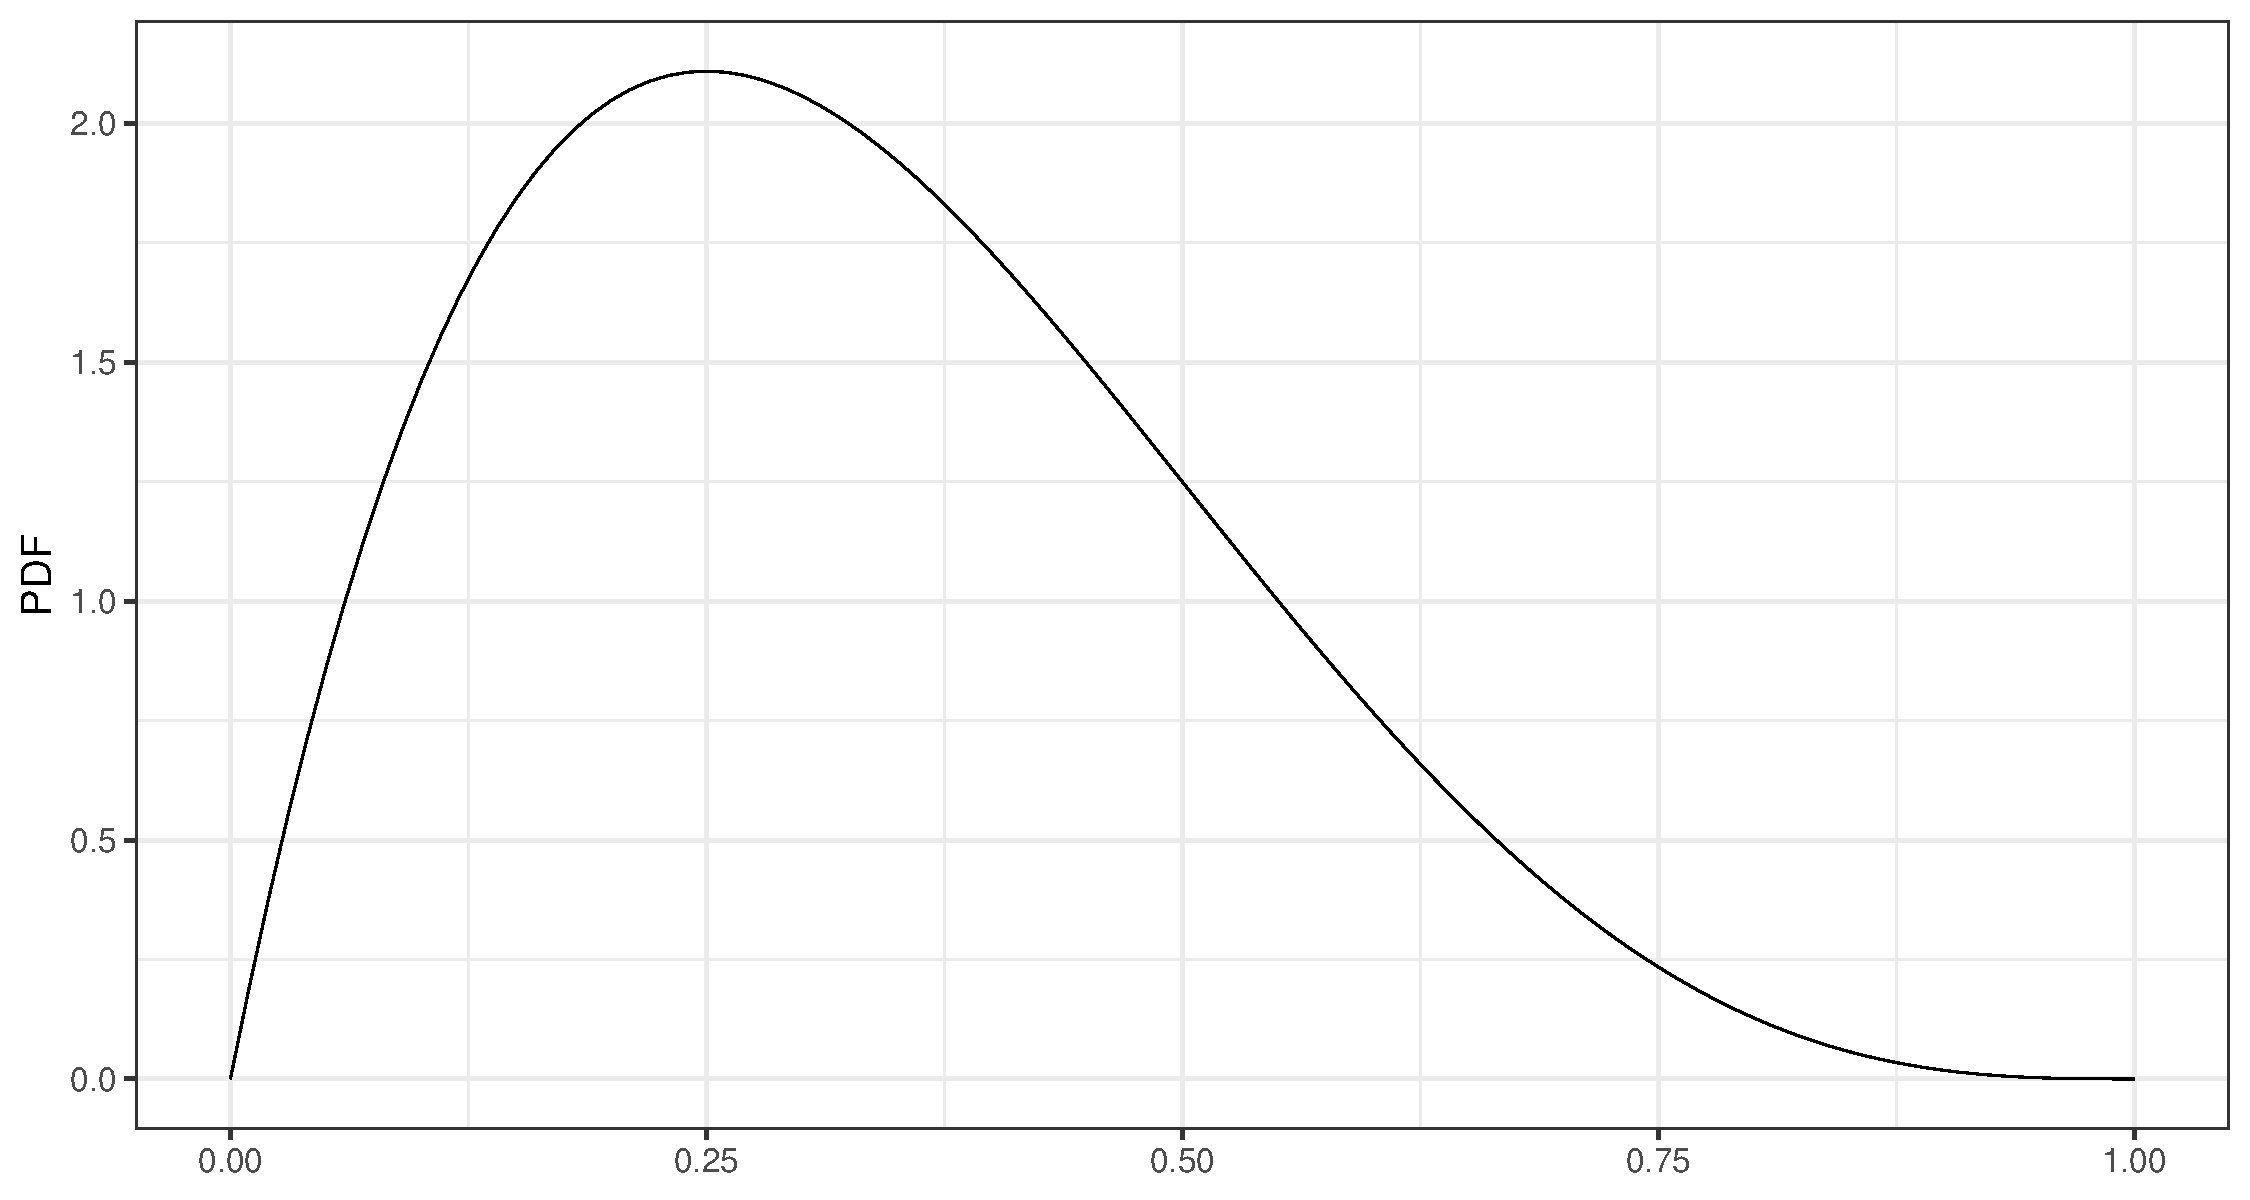
\includegraphics[width=\textwidth]{figure_08.pdf}
	\caption{Probability density function of the beta distribution $\Beta(\alpha, \beta)$
			 with shape parameters $\alpha = 2$ and $\beta = 4$}
	\label{fig:beta_pdf}
\end{figure}

For each model and bias-aware inference procedure we report the average bandwidth,
approximated bias and root MSE, empirical coverage and average interval length across 5000 replications.
We consider the following eight specifications:
Undersmoothing (ad hoc) by dividing the estimated MSE-optimal bandwidth by two and three,
robust bias-correction with bandwidths $\hat{h}_{\text{MSE}}$ and $\hat{h}_{\text{CE}}$,
and the approach by \textcite{Armstrong_2020} with the minimax MSE-optimal and length-optimal bandwidth
(respectively for the rule of thumb choice of the smoothness constant $M_{\text{ROT}}$ and the truth $\overbar{M}$).
In all cases, we conduct local linear estimation with the triangular kernel.
Standard errors are obtained by heteroskedasticity-robust nearest neighbor (with three as the minimum number of neighbors).
For reference, we also report the infeasible MSE-optimal bandwidth $h_{\text{MSE}}$,
which can be derived because of the known data generating process.
All confidence intervals are computed at the nominal 95\% coverage level. 

\subsection{Results and discussion}

The simulation results are collected in Table~\ref{tab:model1}, Table~\ref{tab:model2} and Table~\ref{tab:model3}.
We begin with Model~1 (\cite{Lee_2008}).
Due to the overall linear shape of $\mu_{1}$, the true MSE-optimal bandwidth $h_{\text{MSE}} = 0.166$ is relatively large.
The estimated version $\hat{h}_{\text{MSE}} = 0.196$ is larger,
and results for RBC in some undercoverage (91.70\%).
The CE-optimal bandwidth is substantially smaller and coverage is slightly improved.
For undersmoothing, bias can be reduced and coverage is similar to RBC with $\hat{h}_{\text{CE}}$,
but with wider confidence intervals (the cost of increased variance).
The results for the minimax MSE bandwidth for the correctly specified $\overbar{M}$ are very close to the CE-optimal RBC results in all aspects,
except for improved coverage of 95.38\%, almost exactly the nominal level.
Since the rule of thumb (ROT) calibrated choice is larger than $\overbar{M}$,
the corresponding bandwidth is smaller (as the maximal bias is larger).
The coverage is even better, at the expense of a slightly increased average interval length.
Results for the length-optimal bandwidth selector are essentially the same.
On balance, undersmoothing and RBC exhibit some degree of undercoverage,
with undersmoothing having on average the widest intervals.
In contrast, all specifications of the procedure by \citeauthor{Armstrong_2020} achieve accurate coverage.      

\renewcommand{\arraystretch}{1.2}
\begin{table}
	\centering
	\captionabove{Simulation results for Model 1 \parencite{Lee_2008} and nominal coverage of 95\%}
	\label{tab:model1}
	\resizebox{\textwidth}{!}{%
		\begin{tabular}{l c c c c c}  
			\toprule
			Approach & Bandwidth & Bias & RMSE & CI coverage [\%] & CI length \\
			\midrule
			Undersmoothing (ad hoc) & & & & & \\
			\quad -- By factor 2                       & 0.098 & 0.005 & 0.082 & 92.60 & 0.297 \\
			\quad -- By factor 3                       & 0.065 & 0.001 & 0.101 & 92.24 & 0.370 \\
			Robust bias-correction & & & & & \\
			\quad -- MSE-optimal                       & 0.196 & 0.019 & 0.064 & 91.70 & 0.246 \\
			\quad -- CE-optimal                        & 0.144 & 0.013 & 0.071 & 92.44 & 0.266 \\
			\citeauthor{Armstrong_2020} & & & & & \\
			\quad -- minimax MSE ($M_{\text{ROT}}$)    & 0.126 & 0.011 & 0.069 & 95.12 & 0.289 \\
			\quad -- minimax MSE ($\overbar{M}$)       & 0.146 & 0.014 & 0.063 & 95.38 & 0.266 \\
			\quad -- Length-optimal ($M_{\text{ROT}}$) & 0.130 & 0.011 & 0.068 & 95.50 & 0.289 \\   
		    \quad -- Length-optimal ($\overbar{M}$)    & 0.150 & 0.015 & 0.062 & 95.66 & 0.266 \\               
			\bottomrule \addlinespace[0.25ex]
			\multicolumn{6}{p{\dimexpr \textwidth+3\tabcolsep}}{\footnotesize \textit{Note}:
			The columns are average bandwidth, approximated bias and root MSE,
			empirical coverage and average interval length across the 5000 replications.
			The infeasible MSE-optimal bandwidth is $h_{\text{MSE}} = 0.166$.
			Results are based on local linear estimation and the triangular kernel.
			For the approach by \citeauthor{Armstrong_2020}, the Hölder class is used with
			$M$ as either the rule of thumb $M_{\text{ROT}}$ ($= 22.399$ on average) or the truth $\overbar{M}=14.36$.}
	\end{tabular}}	
\end{table}
\renewcommand{\arraystretch}{1.0}
\newpage
For the second model \parencite{Ludwig_2007} the infeasible MSE-optimal bandwidth is $h_{\text{MSE}} = 0.082$,
which is half the size compared to Model~1, as expected from looking at the plots in Figure~\ref{fig:simulation_models}.
Again, the estimate $\hat{h}_{\text{MSE}} = 0.1$ is too high ($\approx 20\%$) and the RBC method undercovers by two percentage points.
Unfortunately, undersmoothing led to some numerical instability during the simulations for Model~2.
The number of successful replications was too low to obtain reliable results.
The results for the four specifications of \citeauthor{Armstrong_2020} are similar to each other,
as the ROT estimate of $M$ is close to the true value.
The empirical coverage is by one to two percentage points above the nominal level.
Compared to RBC, we obtain longer confidence intervals,
because the relatively high curvature of $\mu_{2}$ is taken into account by accordingly increased critical values.

The results for Model~3 in Table~\ref{tab:model3} are similar to those for Model~1 in Table~\ref{tab:model1}.
The increased overall curvature translates into somewhat smaller bandwidths.
Now, empirical coverage for the ad hoc undersmoothing is slightly worse,
while it is slightly improved for RBC.
The higher degree of curvature means that the bound on the second derivative $M$ is enlarged,
widening on average the \citeauthor{Armstrong_2020} confidence intervals.
Interestingly, for Model~3 $M_{\text{ROT}}$ is considerably below $\overbar{M}$ and similar to $M_{\text{ROT}}$ for Model~1.
This bias of $M_{\text{ROT}}$, however, does not have a relevant impact on coverage (but tightens the intervals).       

\renewcommand{\arraystretch}{1.2}
\begin{table}[p]
	\centering
	\captionabove{Simulation results for Model 2 \parencite{Ludwig_2007} and nominal coverage of 95\%}
	\label{tab:model2}
	\resizebox{\textwidth}{!}{%
		\begin{tabular}{l c c c c c}  
			\toprule
			Approach & Bandwidth & Bias & RMSE & CI coverage [\%] & CI length \\
			\midrule
			Undersmoothing (ad hoc) & & & & & \\
			\quad -- By factor 2                       & 0.050 & NA & NA & NA & NA \\
			\quad -- By factor 3                       & 0.033 & NA & NA & NA & NA \\
			Robust bias-correction & & & & & \\
			\quad -- MSE-optimal                       & 0.100 & 0.048 & 0.098 & 92.98 & 0.345 \\
			\quad -- CE-optimal                        & 0.073 & 0.027 & 0.100 & 93.02 & 0.396 \\
			\citeauthor{Armstrong_2020} & & & & & \\
			\quad -- minimax MSE ($M_{\text{ROT}}$)    & 0.077 & 0.032 & 0.095 & 96.08 & 0.440 \\
			\quad -- minimax MSE ($\overbar{M}$)       & 0.075 & 0.031 & 0.095 & 96.62 & 0.447 \\
			\quad -- Length-optimal ($M_{\text{ROT}}$) & 0.080 & 0.035 & 0.095 & 96.16 & 0.442 \\   
			\quad -- Length-optimal ($\overbar{M}$)    & 0.078 & 0.033 & 0.094 & 96.80 & 0.448 \\               
			\bottomrule \addlinespace[0.25ex]
			\multicolumn{6}{p{\dimexpr \textwidth+3\tabcolsep}}{\footnotesize \textit{Note}:
			The columns are average bandwidth, approximated bias and root MSE,
			empirical coverage and average interval length across the 5000 replications.
			The infeasible MSE-optimal bandwidth is $h_{\text{MSE}} = 0.082$.
			Results are based on local linear estimation and the triangular kernel.
			For the approach by \citeauthor{Armstrong_2020}, the Hölder class is used with
			$M$ as either the rule of thumb $M_{\text{ROT}}$ ($= 103.418$ on average) or the truth $\overbar{M}=109.62$.
			Undersmoothing led to numerical instability, wherefore results are not available.}
	\end{tabular}}	
\end{table}
\renewcommand{\arraystretch}{1.0}

\renewcommand{\arraystretch}{1.2}
\begin{table}[p]
	\centering
	\captionabove{Simulation results for Model 3 and nominal coverage of 95\%}
	\label{tab:model3}
	\resizebox{\textwidth}{!}{%
		\begin{tabular}{l c c c c c}  
			\toprule
			Approach & Bandwidth & Bias & RMSE & CI coverage [\%] & CI length \\
			\midrule
			Undersmoothing (ad hoc) & & & & & \\
			\quad -- By factor 2                       & 0.087 & $-$0.004 & 0.086 & 91.90 & 0.314 \\
			\quad -- By factor 3                       & 0.058 & $-$0.003 & 0.107 & 91.76 & 0.393 \\
			Robust bias-correction & & & & & \\
			\quad -- MSE-optimal                       & 0.173 & $-$0.013 & 0.065 & 92.94 & 0.252 \\
			\quad -- CE-optimal                        & 0.127 & $-$0.006 & 0.072 & 92.96 & 0.275 \\
			\citeauthor{Armstrong_2020} & & & & & \\
			\quad -- minimax MSE ($M_{\text{ROT}}$)    & 0.119 & $-$0.007 & 0.071 & 95.94 & 0.301 \\
			\quad -- minimax MSE ($\overbar{M}$)       & 0.095 & $-$0.005 & 0.079 & 95.64 & 0.339 \\
			\quad -- Length-optimal ($M_{\text{ROT}}$) & 0.122 & $-$0.007 & 0.070 & 96.14 & 0.301 \\   
			\quad -- Length-optimal ($\overbar{M}$)    & 0.098 & $-$0.005 & 0.077 & 96.08 & 0.339 \\               
			\bottomrule \addlinespace[0.25ex]
			\multicolumn{6}{p{\dimexpr \textwidth+3\tabcolsep}}{\footnotesize \textit{Note}:
			The columns are average bandwidth, approximated bias and root MSE,
			empirical coverage and average interval length across the 5000 replications.
			The infeasible MSE-optimal bandwidth is $h_{\text{MSE}} = 0.260$.
			Results are based on local linear estimation and the triangular kernel.
			For the approach by \citeauthor{Armstrong_2020}, the Hölder class is used with
			$M$ as either the rule of thumb $M_{\text{ROT}}$ ($= 26.629$ on average) or the truth $\overbar{M}=45.406$.}
	\end{tabular}}	
\end{table}
\renewcommand{\arraystretch}{1.0}

We summarize the Monte Carlo study as follows.
Undersmoothing achieves a decent coverage, but overall offers the worst combination of coverage and average interval length.
Robust bias-correction undercovers the true treatment effect slightly (similar to undersmoothing),
but yields the shortest intervals.
The CE-optimal bandwidth choice offers some small refinements in empirical coverage relative to the MSE-optimal bandwidth selector.
The best coverage is obtained for the procedure of \citeauthor{Armstrong_2020}.
The global polynomial rule of thumb to choose the required smoothness constant $M$ works reasonably well.
Still, the necessity to specify this constant to bound the second derivative on both sides of the cutoff constitutes a drawback.
Each method, however, imposes (explicitly or implicitly) restrictions on the smoothness of the conditional expectation function.
Estimating the bias in RBC via local quadratic regression assumes that (in a neighborhood around the cutoff)
the regression functions are three times continuously differentiable.
The Monte Carlo experiment suggests to report in practice the confidence intervals of \citeauthor{Armstrong_2020},
$\text{CI}_{\text{AK}}(h^{\text{AK}}_{\text{MSE}}, M_{\text{ROT}})$ and $\text{CI}_{\text{AK}}(h^{\text{AK}}_{\text{CIL}}, M_{\text{ROT}})$,
together with the robust bias-corrected confidence intervals,  
$\text{CI}_{\text{RBC}}(\hat{h}_{\text{MSE}})$ and $\text{CI}_{\text{RBC}}(\hat{h}_{\text{CE}})$.
In doing so, we can likely complement a more accurate but wider interval with a tighter but less accurate interval.
The sensitivity of the confidence intervals to the choice of the bandwidth and smoothing constant can then be further examined.